\documentclass[a4paper,11pt]{article}
\usepackage{ngerman}
\usepackage[utf8]{inputenc} %Umlaute (Mac)
\usepackage{amsmath}
\usepackage{tikzsymbols}
\usepackage{mathtools}
\usepackage{amssymb}
\usepackage{graphicx} 
\usepackage{epstopdf}
\usepackage{fancybox,color}
\usepackage[shortlabels]{enumitem}
\usepackage{caption}
\usepackage{multicol}
\usepackage{floatrow}
\usepackage{dsfont}
\usepackage{bigints}
\usepackage[ruled]{algorithm2e}
\usepackage{hyperref}
% RZ-Makros.TEX
% Dies sind Makros, die f�r alle mathematischen Texte gut sind.

\sloppy
\renewcommand{\thefootnote}{\fnsymbol{footnote}}
\renewcommand{\labelenumi}{(\alph{enumi})}
\renewcommand{\labelenumii}{(\roman{enumii})}
\renewcommand{\labelenumiii}{(\arabic{enumiii})}

%  Allgemeine Makros

\newcommand{\R}{\mathrm{I\!R}}
\newcommand{\N}{\mathrm{I\!N}}
\newcommand{\HH}{\mathrm{I\!H}}
\newcommand{\F}{\mathrm{I\!F}}
\newcommand{\E}{\mathrm{I\!E}}
\newcommand{\K}{\mathrm{I\!K}}
\newcommand{\PP}{\mathrm{I\!P}}

\newcommand{\V}{\mathbb{V}}
\newcommand{\cB}{\mathcal{B}}

\newcommand{\Z}{\mathchoice {\hbox{$\sf\textstyle Z\kern-0.4em
Z$}}{\hbox{$\sf\textstyle Z\kern-0.4em Z$}}{\hbox{$\sf\scriptstyle
Z\kern-0.3em Z$}}{\hbox{$\sf\scriptscriptstyle Z\kern-0.2em Z$}}}

\newcommand{\Q}{\mathchoice {\setbox0=\hbox{$\displaystyle\rm
Q$}\hbox{\raise0.15\ht0\hbox to0pt{\kern0.4\wd0\vrule
height0.8\ht0\hss}\box0}}{\setbox0=\hbox{$\textstyle\rm
Q$}\hbox{\raise0.15\ht0\hbox to0pt{\kern0.4\wd0\vrule
height0.8\ht0\hss}\box0}}{\setbox0=\hbox{$\scriptstyle\rm
Q$}\hbox{\raise0.15\ht0\hbox to0pt{\kern0.4\wd0\vrule
height0.7\ht0\hss}\box0}}{\setbox0=\hbox{$\scriptscriptstyle\rm
Q$}\hbox{\raise0.15\ht0\hbox to0pt{\kern0.4\wd0\vrule
height0.7\ht0\hss}\box0}}}

\newcommand{\C}{\mathchoice {\setbox0=\hbox{$\displaystyle\rm
C$}\hbox{\hbox to0pt{\kern0.4\wd0\vrule
height0.9\ht0\hss}\box0}}{\setbox0=\hbox{$\textstyle\rm C$}\hbox{\hbox
to0pt{\kern0.4\wd0\vrule
height0.9\ht0\hss}\box0}}{\setbox0=\hbox{$\scriptstyle\rm C$}\hbox{\hbox
to0pt{\kern0.4\wd0\vrule
height0.9\ht0\hss}\box0}}{\setbox0=\hbox{$\scriptscriptstyle\rm
C$}\hbox{\hbox to0pt{\kern0.4\wd0\vrule height0.9\ht0\hss}\box0}}}

\newcommand{\OO}{\mathchoice {\setbox0=\hbox{$\displaystyle\rm
O$}\hbox{\hbox to0pt{\kern0.4\wd0\vrule
height0.9\ht0\hss}\box0}}{\setbox0=\hbox{$\textstyle\rm O$}\hbox{\hbox
to0pt{\kern0.4\wd0\vrule
height0.9\ht0\hss}\box0}}{\setbox0=\hbox{$\scriptstyle\rm O$}\hbox{\hbox
to0pt{\kern0.4\wd0\vrule
height0.9\ht0\hss}\box0}}{\setbox0=\hbox{$\scriptscriptstyle\rm
O$}\hbox{\hbox to0pt{\kern0.4\wd0\vrule height0.9\ht0\hss}\box0}}}

\newcommand{\scrA}{\mathcal{A}}
\newcommand{\scrB}{\mathcal{B}}
\newcommand{\scrC}{\mathcal{C}}
\newcommand{\scrD}{\mathcal{D}}
\newcommand{\scrE}{\mathcal{E}}
\newcommand{\scrF}{\mathcal{F}}
\newcommand{\scrG}{\mathcal{G}}
\newcommand{\scrH}{\mathcal{H}} % alt \Hscr
\newcommand{\scrI}{\mathcal{I}}
\newcommand{\scrJ}{\mathcal{J}}
\newcommand{\scrK}{\mathcal{K}}
\newcommand{\scrL}{\mathcal{L}}
\newcommand{\scrM}{\mathcal{M}}
\newcommand{\scrN}{\mathcal{N}}
\newcommand{\scrO}{\mathcal{O}}
\newcommand{\scrP}{\mathcal{P}}
\newcommand{\scrQ}{\mathcal{Q}}
\newcommand{\scrR}{\mathcal{R}}
\newcommand{\scrS}{\mathcal{S}}
\newcommand{\scrT}{\mathcal{T}}
\newcommand{\scrU}{\mathcal{U}}
\newcommand{\scrV}{\mathcal{V}} % alt \Vscr
\newcommand{\scrW}{\mathcal{W}}
\newcommand{\scrX}{\mathcal{X}}
\newcommand{\scrY}{\mathcal{Y}}
\newcommand{\scrZ}{\mathcal{Z}}


%% Es werden Fu�not-Symbolgleichungsnummerierung und Normal-Gleichungsnummerierung
%% eingef�hrt. Die Z�hler sind seqcounter und neqcouter. In jedem neuen Abschnitt
%% beginnt die Z�hlung von vorne
\newcounter{neqcounter}[section]
\newcounter{seqcounter}[section]
\newcommand{\numberequation}[1]
   {\renewcommand{\theequation}{\arabic{equation}}
    \setcounter{equation}{\value{neqcounter}}
    \begin{equation}#1\end{equation}\stepcounter{neqcounter}}
\newcommand{\symbolequation}[1]
   {\renewcommand{\theequation}{\fnsymbol{equation}}
    \setcounter{equation}{\value{seqcounter}}
    \begin{equation}#1\end{equation}\stepcounter{seqcounter}}

\newcommand{\diff}{\mathrm{d}}
\newcommand{\Diff}{\mathrm{D}}
\newcommand{\id}{\mathrm{id}}
\newcommand{\GL}{\mathrm{GL}}
\newcommand{\SL}{\mathrm{SL}}
\newcommand{\SO}{\mathrm{SO}}
\newcommand{\End}{\mathrm{End}}
\newcommand{\Alt}{\mathrm{Alt}}
\newcommand{\Spur}{\mathrm{Spur}}
\newcommand{\rk}{\mathrm{rk}}
\newcommand{\rg}{\mathrm{rg}}
\newcommand{\Spann}{\mathrm{Spann}}
\newcommand{\Top}{\mathrm{Top}}
\newcommand{\del}{\partial}
\newcommand{\ddel}[2]{\frac{\partial#1}{\partial#2}}
\newcommand{\ddeldel}[3]{\frac{\partial^2#1}{\partial#2\:\partial#3}}
\newcommand{\ddelsquare}[2]{\frac{\partial^2#1}{\partial{#2}^2}}
\newcommand{\grad}{\mathrm{grad}}
\newcommand{\hess}{\mathrm{hess}}
\newcommand{\Hess}{\mathrm{Hess}}
\newcommand{\Rp}{\R_+}
\newcommand{\eps}{\varepsilon}
\newcommand{\vi}{\varphi}
\newcommand{\vkap}{\varkappa}
\newcommand{\thet}{\vartheta}
\newcommand{\UL}{\mathchoice
{\setbox0=\hbox{$\displaystyle U$}
 \setbox1=\hbox{$\displaystyle l$}
 \hbox{\box0\kern-0.80\wd1\lower0.029\ht1\box1}}
{\setbox0=\hbox{$\displaystyle U$}
 \setbox1=\hbox{$\displaystyle l$}
 \hbox{\box0\kern-0.80\wd1\lower0.029\ht1\box1}}
{\setbox0=\hbox{$\scriptstyle U$}
 \setbox1=\hbox{$\scriptstyle l$}
 \hbox{\box0\kern-0.80\wd1\lower0.029\ht1\box1}}
{\setbox0=\hbox{$\scriptscriptstyle U$}
 \setbox1=\hbox{$\scriptscriptstyle l$}
 \hbox{\box0\kern-0.80\wd1\lower0.029\ht1\box1}}
}

\newcommand{\Uo}{\UL^o}
\def\fam#1#2#3#4{({#1}_{#2})_{#2=#3,\dotsc,#4}}
\def\zz#1#2#3{#1=#2,\dotsc,#3}
\newcommand{\intint}[2]{\{#1,\dotsc,#2\}}
\newcommand{\Vektor}[2]{({#1}_1,\dotsc,{#1}_{#2})} 

\newcommand{\qmq}[1]{\quad\mbox{#1}\quad}
\newcommand{\Menge}[2]{\{\,#1\,|\,#2\,\}}
\newcommand{\Abstand}[1]{\mbox{}\par\vspace{-#1mm}}

\def\bild#1#2#3#4{\leavevmode\vbox to #1{\vfil \hbox to #2{\special{picture #4
   scaled #3}\hfil}}}
   %Parametr: #1=H�he,#2=Breite,#3=Skalierung 0.1<f<10,#4=Bildname

%%  Zu den Rahmen:
%%  grRahmen ist mit rahmen aus dem Alalysisscript identisch.
%%  grRahmen geht fast �ber die ganze Textbreite
%%
%%  klRahmen ist aus kleinerRahmen aus den RZ-Makros von 1996 entstanden;
%%  seine H�he ist etwas vergr��ert worden,
%%  seine Breite ist dem Text angepasst, dieser darf nur eine Zeile sein
%%
%%  varRahmen ist eine Neusch�pfung: Man stellt eine Breite ein. Dann wird der
%%  in dem Rahmen wie in einer Minipage behandelt.
%%
\newcommand{\grRahmen}[1]{\begin{center}\setlength{\fboxrule}{0.8pt}
           \setlength{\fboxsep}{8pt}
              \fbox{\begin{minipage}{140mm}\rule{0mm}{5mm}\hspace*{-2mm} #1
                    \end{minipage}}\end{center}}

\newcommand{\klRahmen}[1]{\begin{center}\large\setlength{\fboxrule}{0.8pt}
                     \setlength{\fboxsep}{8pt}
                     \fbox{\rule[-2mm]{0mm}{7mm} #1 }
                     \normalsize\end{center}}

\newcommand{\varRahmen}[2]{\begin{center}\setlength{\fboxrule}{0.8pt}
           \setlength{\fboxsep}{8pt}
              \fbox{\begin{minipage}{#1}\rule{0mm}{5mm}\hspace*{-2mm} #2
                    \end{minipage}}\end{center}}

% die 1996-Version
%\newcommand{\kleinerRahmen}[1]{\begin{center}\large\setlength{\fboxrule}{0.8pt}
%                     \setlength{\fboxsep}{8pt}\fbox{#1}\normalsize\end{center}}

%% Randnotizen vom Juli 1997
\setlength{\marginparsep}{5pt}
\setlength{\marginparwidth}{30pt}
\newcommand{\marginlabel}[1]           
                 {\mbox{}\marginpar{\raggedleft\hspace{0pt}#1}}
\newcommand{\Ausrufezeichen}{\marginlabel{\raisebox{-1.2ex}{\Huge$\boldsymbol{!}$}}}
\newcommand{\Randbalken}[2]{\marginlabel{{\rule[#1]{0.5mm}{#2}}}}
\newcommand{\Zeigefinger}{\marginlabel{\raisebox{-0.8ex}{\LARGE\ding{43}}}}
\newcommand{\Blume}{\marginlabel{\raisebox{-0.6ex}{\LARGE\ding{94}}}}

%  Differentialgeometrie - Makros
\newcommand{\bigoperp}{\mathop{\bigcirc\raisebox{0.25em}
 {\hskip-0.53em\hbox{\vrule height1.0ex width0.04em}
  \hskip-0.77em\hbox{\vrule height0.04em width 0.8em}
  \hskip- 0.2em}}}

\renewcommand{\bigoplus}{\mathop{\bigcirc
  \raisebox{-0.22em}{\hskip-0.53em\hbox{\vrule height2.08ex width0.04em}
  \raisebox{ 0.48em}{\hskip-0.75em\hbox{\vrule height0.04em width 0.8em}}
  \hskip- 0.2em}}}

\def\NP#1#2#3{\mathchoice
  {{\textstyle{\prod\limits_{i=#2}^{#3}}{#1}_i}} 
  {{\textstyle{\prod_{i=#2}^{#3}}{#1}_i}}
  {}
  {}
   }
\def\DS#1#2#3{\bigoplus_{i=#2}^{#3}\!#1_i} 
\def\OS#1#2#3{\bigoperp_{i=#2}^{#3}#1_i} 
\def\WP#1#2#3{#1_0 \times_{#2}\NP {#1}{1}{#3}}
\def\TP#1#2#3#4{{\rule{0mm}{2ex}}^{#2}\NP{#1}{#3}{#4}}

\newcommand {\cinf}{\ensuremath{\mathrm{C}^{\infty}}}
\newcommand {\X}{\mathfrak{X}}
\newcommand{\Tensor}[3]{\mathfrak{T}^{(#2,#3)}(#1)}
\newcommand{\alphad}{\dot{\alpha}}
\newcommand {\g}[2]{\langle #1,#2\rangle}
\def\gg{\g{\cdot}{\cdot}}
\newcommand {\euc}[2]{\langle\!\langle #1,#2 \rangle\!\rangle}
\newcommand {\peuc}[2]{\langle\!\langle #1,#2 \rangle\!\rangle\!_s}
\newcommand {\Kov}[2]{\nabla_{#1}#2}
\newcommand {\Kovh}[2]{\widehat{\nabla}_{#1}#2}
\newcommand {\Kovt}[2]{\widetilde{\nabla}_{#1}#2}
\newcommand {\Kovperp}[2]{\nabla^{\perp}_{#1}#2}
\newcommand {\Kovv}[3]{{\nabla^{\scriptscriptstyle{#1}}}_{\!#2}#3}
\newcommand {\operp}{\mathbin{\mbox{$\ominus\raisebox{2.9pt}
 {\hskip-0.42em\hbox{\vrule height0.7ex width0.02em}\hskip0.42em }$}}}
\newcommand {\TpM}{T_{p}M}
\newcommand {\Tpf}{T_{p}f}
\newcommand {\Nf}{\perp\!\!(f)}
\newcommand {\NM}{\perp\!\!M}
\newcommand {\Npf}{\perp_p\!\!(f)}
\newcommand {\NpM}{\perp_p\!\!M}
\newcommand {\Nepf}{\perp^{\!\!1}_p\!\!(f)}
\newcommand {\NepM}{\perp^{\!\!1}_p\!\!M}
\newcommand{\Shop}[3]{{\mathrm{A}^{^{\scriptscriptstyle{\!\!#1}}}_{#2}}#3} %shape op

% Horizontale/vertikale VR 
%\def\Vscr{\mathcal{V}}   ersetzt durch \scrV
%\def\Hscr{\mathcal{H}}   ersetzt durch \scrH
%\def\Vscrt{\widetilde{\mathcal{V}}}  ersetzt durch
\def\tscrV{\widetilde{\mathcal{V}}}
%\def\Hscrt{\widetilde{\mathcal{H}}}  ersetzt durch
\def\tscrH{\widetilde{\mathcal{H}}}
\newcommand{\hdisp}[3]{\overset{#2}{\underset{#1}{\parallel}}\!\!#3\,} 
    % horicontal displacement
\newcommand{\Hol}{\mathrm{Hol}}

% Reelle projektive R�ume
\newcommand {\RPn}{\ensuremath{\R\mathrm{P}^{n}}}
\newcommand {\RPm}{\ensuremath{\R\mathrm{P}^{m}}}

\newcommand {\cA}{\mathcal{A}}
% Komplexe Raumformen
\newcommand {\CPn}{\ensuremath{\C\mathrm{P}^{n}}}
\newcommand {\CPm}{\ensuremath{\C\mathrm{P}^{m}}}
\newcommand {\CHn}{\ensuremath{\C\mathrm{H}^{n}}}
\newcommand {\CHm}{\ensuremath{\C\mathrm{H}^{m}}}

\def\Mgf/{Mannigfaltigkeit}
\def\UMgf/{Untermannigfaltigkeit}
\def\Abb/{Abbildung}
\def\zshgd/{zusammenh�ngend}
\def\FR/{Faserraum}
\def\FB/{Faserb�ndel}
\def\VB/{Vektorb�ndel}
\def\UVB/{Untervektorb�ndel}

\hyphenation{Riemann-sche Riemann-ian}

\endinput
% Ende von RZ-Makros.TEX


% SKK-Makros.TEX
% Dies sind Makros, die f�r alle mathematischen Texte gut sind.

% Aus Article_G&E_11pt, von sk modifiziert 9.3.2004
\setlength{\textheight}{23cm}
\setlength{\textwidth}{16cm}
\setlength{\oddsidemargin}{0.2cm}
\setlength{\evensidemargin}{0.2cm}
\setlength{\topmargin}{0cm}
\setlength{\headheight}{0cm}
\setlength{\topsep}{0pt}
\setlength{\headsep}{1.0cm}
\setlength{\partopsep}{0pt}
\parindent0pt
\setlength{\parskip}{0.7\baselineskip}

% Alter Stand
%\setlength{\parindent}{0pt}
%%%%\setlength{\parskip}{2ex plus 0.5ex minus 0.3ex}
%\setlength{\parskip}{0.7\baselineskip}
%\setlength{\topmargin}{0cm}
%\setlength{\headheight}{3ex}
%\textwidth 16cm
%\setlength{\oddsidemargin}{7mm}
%\setlength{\evensidemargin}{-0.5mm}
%\setlength{\textheight}{22cm}
%\topsep0pt
%\partopsep0pt

\pagestyle{headings}

\newcommand{\clearemptydoublepage}{\newpage{\pagestyle{empty}\cleardoublepage}}

\newcommand{\cF}{\mathcal{F}}
\newcommand{\cS}{\mathcal{S}}
\newcommand{\cR}{\mathcal{R}}
\newcommand{\ggT}{\mathrm{ggT}}
\newcommand{\vol}{\mathop{\mathrm{vol}}\nolimits}
\newcommand{\sign}{\mathop{\mathrm{sign}}\nolimits}
%\newcommand{\rk}{\mathop{\mathrm{rk}}\nolimits}
%\newcommand{\rg}{\mathop{\mathrm{rg}}\nolimits}
\newcommand{\rang}{\mathop{\mathrm{rang}}\nolimits}
\newcommand{\Og}{\mathrm{O}}
\newcommand{\Ug}{\mathrm{U}}
\newcommand{\SU}{\mathrm{SU}}
\newcommand{\Sp}{\mathrm{Sp}}
\newcommand{\PGL}{\mathrm{PGL}}
\newcommand{\PU}{\mathrm{PU}}
\newcommand{\Lg}{\mathrm{L}}
\newcommand{\Lin}{\mathrm{Lin}}
\newcommand{\Spin}{\mathrm{Spin}}
\newcommand{\Pin}{\mathrm{Pin}}
\newcommand{\Der}{\mathrm{Der}}
\newcommand{\RE}{\mathop{\mathrm{Re}}\nolimits}
\newcommand{\IM}{\mathop{\mathrm{Im}}\nolimits}
\newcommand{\Kern}{\mathop{\mathrm{Kern}}\nolimits}
\newcommand{\Rang}{\mathop{\mathrm{Rang}}\nolimits}
\newcommand{\Eig}{\mathop{\mathrm{Eig}}\nolimits}
\newcommand{\Aut}{\mathop{\mathrm{Aut}}\nolimits}
\newcommand{\AAut}{\overline{\Aut}}
\newcommand{\Bij}{\mathop{\mathrm{Bij}}\nolimits}
\newcommand{\ad}{\mathop{\mathrm{ad}}\nolimits}
\newcommand{\Ad}{\mathop{\mathrm{Ad}}\nolimits}
\newcommand{\Exp}{\mathop{\mathrm{Exp}}\nolimits}
\newcommand{\Fix}{\mathop{\mathrm{Fix}}\nolimits}
\newcommand{\spn}{\mathop{\mathrm{span}}\nolimits}
\newcommand{\tr}{\mathop{\mathrm{tr}}\nolimits}
\newcommand{\Spec}{\mathop{\mathrm{Spec}}\nolimits}
\newcommand{\even}{\mathrm{even}}
\newcommand{\odd}{\mathrm{odd}}
\newcommand{\pr}{\mathrm{pr}}
\newcommand{\ric}{\mathop{\mathrm{ric}}\nolimits}
\newcommand{\Ric}{\mathop{\mathrm{Ric}}\nolimits}
\newcommand{\Geins}{\mathrm{G1}}
\newcommand{\Gzwei}{\mathrm{G2}}
\newcommand{\Gdrei}{\mathrm{G3}}
\newcommand{\Peins}{\mathrm{P1}}
\newcommand{\Pzwei}{\mathrm{P2}}
\newcommand{\Atyp}{\mathrm{A}}
\newcommand{\Ieins}{\mathrm{I1}}
\newcommand{\Izwei}{\mathrm{I2}}
\newcommand{\diam}{\mathop{\mathrm{diam}}\nolimits}

\newcommand{\A}{\mathfrak{A}}
\newcommand{\liea}{\mathfrak{a}}
\newcommand{\lieb}{\mathfrak{b}}
\newcommand{\liec}{\mathfrak{c}}
\newcommand{\lieaut}{\mathfrak{aut}}
\newcommand{\lief}{\mathfrak{f}}
\newcommand{\lieg}{\mathfrak{g}}
\newcommand{\liei}{\mathfrak{i}}
\newcommand{\liegl}{\mathfrak{gl}}
\newcommand{\lieh}{\mathfrak{h}}
\newcommand{\liej}{\mathfrak{j}}
\newcommand{\liek}{\mathfrak{k}}
\newcommand{\liel}{\mathfrak{l}}
\newcommand{\liem}{\mathfrak{m}}
\newcommand{\lieo}{\mathfrak{o}}
\newcommand{\liesl}{\mathfrak{sl}}
\newcommand{\lieso}{\mathfrak{so}}
\newcommand{\liesp}{\mathfrak{sp}}
\newcommand{\lieu}{\mathfrak{u}}
\newcommand{\liesu}{\mathfrak{su}}
\newcommand{\liez}{\mathfrak{z}}
\newcommand{\RP}{\ensuremath{\R\mathrm{P}}}
\newcommand{\CP}{\ensuremath{\C\mathrm{P}}}
\newcommand{\HP}{\ensuremath{\HH\mathrm{P}}}
\newcommand{\OP}{\ensuremath{\OO\mathrm{P}}}
\newcommand{\KP}{\ensuremath{\K\mathrm{P}}}
\newcommand{\CQ}{\ensuremath{\C\mathrm{Q}}}
\newcommand{\ee}{\mathbf{e}}
\newcommand{\EE}{\mathbf{E}}
\newcommand{\PG}{\mathrm{PG}}
\newcommand{\St}{\mathrm{St}}
\newcommand{\VV}{\mathbb{V}}
\newcommand{\TG}{\mathfrak{TG}}
\newcommand{\Geo}{\mathrm{Geo}}
\newcommand{\Kon}{\mathrm{Kon}}
\newcommand{\Con}{\mathrm{Con}}
\newcommand{\Nil}{\mathrm{Nil}}

\newcommand{\frakA}{\mathfrak{A}}
\newcommand{\frakB}{\mathfrak{B}}
\newcommand{\frakC}{\mathfrak{C}}
\newcommand{\frakD}{\mathfrak{D}}
\newcommand{\frakE}{\mathfrak{E}}
\newcommand{\frakF}{\mathfrak{F}}
\newcommand{\frakG}{\mathfrak{G}}
\newcommand{\frakH}{\mathfrak{H}}
\newcommand{\frakI}{\mathfrak{I}}
\newcommand{\frakJ}{\mathfrak{J}}
\newcommand{\frakK}{\mathfrak{K}}
\newcommand{\frakL}{\mathfrak{L}}
\newcommand{\frakM}{\mathfrak{M}}
\newcommand{\frakN}{\mathfrak{N}}
\newcommand{\frakO}{\mathfrak{O}}
\newcommand{\frakP}{\mathfrak{P}}
\newcommand{\frakQ}{\mathfrak{Q}}
\newcommand{\frakR}{\mathfrak{R}}
\newcommand{\frakS}{\mathfrak{S}}
\newcommand{\frakT}{\mathfrak{T}}
\newcommand{\frakU}{\mathfrak{U}}
\newcommand{\frakV}{\mathfrak{V}}
\newcommand{\frakW}{\mathfrak{W}}
\newcommand{\frakX}{\mathfrak{X}}
\newcommand{\frakY}{\mathfrak{Y}}
\newcommand{\frakZ}{\mathfrak{Z}}

\newcommand{\bbA}{\mathbb{A}}
\newcommand{\bbB}{\mathbb{B}}
\newcommand{\bbC}{\mathbb{C}}
\newcommand{\bbD}{\mathbb{D}}
\newcommand{\bbE}{\mathbb{E}}
\newcommand{\bbF}{\mathbb{F}}
\newcommand{\bbG}{\mathbb{G}}
\newcommand{\bbH}{\mathbb{H}}
\newcommand{\bbI}{\mathbb{I}}
\newcommand{\bbJ}{\mathbb{J}}
\newcommand{\bbK}{\mathbb{K}}
\newcommand{\bbL}{\mathbb{L}}
\newcommand{\bbM}{\mathbb{M}}
\newcommand{\bbN}{\mathbb{N}}
\newcommand{\bbO}{\mathbb{O}}
\newcommand{\bbP}{\mathbb{P}}
\newcommand{\bbQ}{\mathbb{Q}}
\newcommand{\bbR}{\mathbb{R}}
\newcommand{\bbS}{\mathbb{S}}
\newcommand{\bbT}{\mathbb{T}}
\newcommand{\bbU}{\mathbb{U}}
\newcommand{\bbV}{\mathbb{V}}
\newcommand{\bbW}{\mathbb{W}}
\newcommand{\bbX}{\mathbb{X}}
\newcommand{\bbY}{\mathbb{Y}}
\newcommand{\bbZ}{\mathbb{Z}}
\newcommand{\gt}{\theta}

\newcommand{\Sph}{\bbS}
\newcommand{\vrprod}[2]{{\textstyle\bigwedge^{#1}\!#2}}
\newcommand{\tenprod}[2]{{\textstyle\bigotimes^{#1}\!#2}}
\newcommand{\spr}[2]{<\!#1,#2\!>}
\newcommand{\sprr}[3]{\spr{#1}{#2}^{(#3)}}
\newcommand{\gR}[2]{\langle #1,#2\rangle_{\R}}
\newcommand{\gC}[2]{\langle #1,#2\rangle_{\C}}
\newcommand{\gH}[2]{\langle #1,#2\rangle_{\HH}}
\newcommand{\gJ}[2]{\langle #1,#2\rangle_{\widetilde{\mathfrak{J}}}}
\newcommand{\gext}[3]{\langle #1,#2 \rangle^{(#3)}}
\newcommand{\Kovr}[3]{\overset{(#1)}{\nabla}_{\!\!#2\,}#3}
\newcommand{\wwedge}{\curlywedge}
\newcommand{\card}[1]{\mathtt{\#}#1}
\newcommand{\offeneaussage}{\ensuremath{\,\Diamond\,}}
\newcommand{\beweis}{\emph{Proof. }}
\newcommand{\beweisende}{\strut\hfill $\Box$\par\medskip}
\newcommand{\Mengegr}[2]{\{\,#1\,{\bigr |}\,#2\,\}}
\newcommand{\ns}[1]{\perp\nobreak\!\nobreak\!\nobreak #1}		% "normal space"
\newcommand{\uns}[1]{\perp^1\nobreak\!\nobreak\!\nobreak #1}		% "unit normal space"
\newcommand{\nsp}[2]{\perp_{#2}\nobreak\!\nobreak\!\nobreak #1}		% "normal space in p"
\newcommand{\unsp}[2]{\perp^1_{#2}\nobreak\!\nobreak\!\nobreak #1}	% "unit normal space in p"
\newcommand{\ddt}{\frac{\mathrm{d}\;}{\mathrm{d}t}}
\newcommand{\dotddt}{\dot{\ddt}}
\newcommand{\wt}{\widetilde}
\newcommand{\wh}{\widehat}

\renewcommand{\C}{\mathchoice {\setbox0=\hbox{$\displaystyle\rm
C$}\hbox{\hbox to0pt{\kern0.4\wd0\vrule
height0.95\ht0\hss}\box0}}{\setbox0=\hbox{$\textstyle\rm C$}\hbox{\hbox
to0pt{\kern0.4\wd0\vrule
height0.95\ht0\hss}\box0}}{\setbox0=\hbox{$\scriptstyle\rm C$}\hbox{\hbox
to0pt{\kern0.4\wd0\vrule
height0.95\ht0\hss}\box0}}{\setbox0=\hbox{$\scriptscriptstyle\rm
C$}\hbox{\hbox to0pt{\kern0.4\wd0\vrule height0.95\ht0\hss}\box0}}}

\newcommand{\hfilll}{\hskip 0pt plus 1filll}

\newcommand{\winzzaesur}{\bigskip{\Large\strut\ \hfill * \hfill}\bigskip}
\newcommand{\kleinezaesur}{\bigskip{\Huge\strut\ \hfill * \hfill}\bigskip}
\newcommand{\mittlerezaesur}{\bigskip{\Huge\strut\ \hfill * * \hfill}\bigskip}
\newcommand{\grossezaesur}{\bigskip{\Huge\strut\ \hfill * * * \hfill}\bigskip}

\newenvironment{myboxed}[0] %
{\begin{boxedminipage}[t]{\textwidth}} %
{\end{boxedminipage}}

\newcounter{prtemp}
\newcommand{\prenumi}[1]{(\alph{#1})}
\newcommand{\refenumi}[1]{\setcounter{prtemp}{\ref{#1}}\prenumi{prtemp}}
\renewcommand{\labelenumi}{\prenumi{enumi}}

\newlength{\doubleboxwidth}
\setlength{\doubleboxwidth}{\textwidth}
\addtolength{\doubleboxwidth}{-0.35cm}

{
\selectlanguage{english}
\hyphenation{Grass-mann-ian}
\hyphenation{Rie-mann-ian}
\hyphenation{geo-me-try}
\hyphenation{ho-lo-morph ho-lo-mor-phic}
\hyphenation{mani-fold mani-folds sub-mani-fold sub-mani-folds}
\hyphenation{sub-mani-fold sub-mani-folds}
\hyphenation{ana-log-ous ana-log-ous-ly}
\hyphenation{ele-ment ele-ments}
\hyphenation{or-tho-go-nal}
\hyphenation{cor-res-pond cor-res-ponding cor-res-pon-dence}
\hyphenation{com-plexifi-ca-tion}
\hyphenation{iso-me-try iso-me-tries}
}

{
\selectlanguage{german}
\hyphenation{Rie-mann sym-me-tri-schen Trans-vek-tions-gruppe}
}


\pagestyle{plain} %erg�nzt
\baselineskip 1ex
\parskip 2ex
\oddsidemargin -0.5cm% Aus 0.5 eine -0.5
\topmargin 0cm       % Aus 3 eine 0, Druckertreiber #1
\headheight 0cm
\headsep 0cm
%\topskip 0cm
\textheight 24cm     % Aus 23 eine 24
\textwidth 17cm      % Aus 15 eine 17
\footskip 1 cm
\setlength{\jot}{4.5pt}
\renewcommand{\baselinestretch}{1.2}% Aus 1.2 eine 1.1

%\renewcommand{\labelenumi}{\large \bf \arabic{enumi}.}%Aus Large ein large
%\renewcommand{\labelenumii}{(\bf \alph{enumii})}
%\renewcommand{\labelenumiii}{(\bf \roman{enumiii})}
%\renewcommand{\labelenumiv}{(\bf \Alph{enumiv}.}

%\renewcommand{\labelenumi}{\large \bf \arabic{enumi}.}%Aus Large ein large
%\renewcommand{\labelenumii}{(\bf \roman{enumii})}
%\renewcommand{\labelenumiii}{(\bf \alph{enumiii})}

\renewcommand{\labelenumi}{\large \bf \arabic{enumi}.}%Aus Large ein large
\renewcommand{\labelenumii}{\bf (\alph{enumii})}
\renewcommand{\labelenumiii}{\bf (\roman{enumiii})}

\newcommand{\nequiv}{\equiv\hspace{-10pt}/\hspace{6pt}}
\newcommand{\oarrowint}%
{\raisebox{1.5pt}{$\scriptscriptstyle\wedge$}%
\hspace{-14.7pt}\bigcirc\hspace{-13pt}  \int}

\newcommand{\aufg}[1]{\phantom{x}\vspace{1.5ex}\noindent {\large\bf\sffamily {#1}.}}

\newcommand{\weitermitaufgabe}[1]{\setcounter{enumi}%
{#1}\addtocounter{enumi}{-1}}

\newcommand{\blatt}[1]{\setcounter{enumi}%
	{#1}\addtocounter{enumi}{-1}}

\newcommand{\naechsteaufgabe}{\bigskip}
\def \m {{\bf m.}\,\,}
\def \s {{}\,\,{\bf s.}\,\,\,}
\newcommand{\Aufgabe}{\bigskip\item}

\DeclareMathAlphabet{\Set}{U}{eur}{m}{n}

\newenvironment{minipageenumerate}%
{\hspace{-4.5mm}\begin{minipage}[t]{15.9cm}\Abstand{9}\begin{enumerate}}%
{\end{enumerate}\end{minipage}}
%\newcommand{\Abstand}[1]{\mbox{}\par\vspace{#1pt}}


\usepackage{tikz}
\usetikzlibrary{arrows, positioning}
\usepackage[pdftex]{pict2e}

\newcommand{\unity}{{1\!\!\!\:\mathrm{l}}}
\newcommand{\Reg}{\operatorname{Reg}}
\newcommand{\kompRe}{\operatorname{Re}}
\newcommand{\kompIm}{\operatorname{Im}}

\begin{document}
	\vspace*{-1cm}
	\noindent
	\includegraphics[viewport=00 25 270 40,scale=.8]{Dependencies/BK1.eps}	\hfill\includegraphics[height=30pt]{Dependencies/logo_uni_neu.pdf}\\
	\vspace{.05cm}
	\noindent\hrulefill\\
	{Prof. Dr. Leif D"oring} \hfill
	{Stochastik 1}\\
	{Benedikt Wille \strut}  \hfill
	%{17. September 2024} 
	\\ \normalsize
	\noindent\vspace{-1.5cm} 
	\begin{center} {\large \bf
		Kreative Diskussion Woche 2} \\
	\end{center}
	
Wir orientieren uns nach wie vor an den Fragen aus dem letzten Tutorium, deren Beantwortung wir anhand eines Beispiels, des unendlich wiederholten Münzwurfs näherkommen wollen:

\begin{itemize}
    \item Warum wollen wir nicht immer mit der Potenzmenge $\mathbb{P}(\Omega)$ als $\sigma$-Algebra modellieren? Was wollen wir stattdesssen verwenden?
    \item Warum sollten wir in der Definition der $\sigma$-Algebren auch (abzählbar) unendliche Vereinigungen zulassen? (Hier wollen wir zumindest eine grobe Idee vermitteln)
\end{itemize}

Eine erste Antwort auf die erste Frage ist dabei, dass wir mit der Potenzmenge als $\sigma$-Algebra nicht einmal das unendlich wiederholte Werfen einer fairen Münze modellieren können (Stichwort Vitali-Mengen) und dass wir stattdessen die Borel-$\sigma$-Algebra verwenden wollen. Heute wollen wir nun ein Maß auf der Borel-$\sigma$-Algebra definieren, das unseren Anforderungen genügt. Das Setting war folgendes:

\begin{itemize}
    \item Raum der Münzwürfe: $\Omega:=\{0,1\}^{\mathbb{N}}:=\{\omega = (\omega_i)_{i\in\mathbb{N}}:\,\omega_i\in\{0,1\}\}$.
    \item \glqq Elementarereignisse\grqq: $\lbrack \omega_1,\dots,\omega_n\rbrack :=\{\Tilde{\omega}\in\Omega:\,\Tilde{\omega}_i=\omega_i\,\forall i=1,\dots,n\}$.
    \item Borel-$\sigma$-Algebra: $\mathcal{B}(E):=\sigma(\mathcal{O})$, $\mathcal{O}$ Menge aller offenen Mengen eines metrischen Raumes $(E,d)$.
    \item Metrik für unseren Raum $\Omega$:
    $$d:\Omega\times\Omega \rightarrow \mathbb{R}_+,\quad (\omega,\Tilde{\omega})\mapsto d(\omega,\Tilde{\omega}):=\begin{cases}
    2^{-\inf\{n\in\mathbb{N}:\,\omega_n\neq\Tilde{\omega}_n\}} &,\omega\neq\Tilde{\omega}\\
    0 &,\omega=\Tilde{\omega}
    \end{cases}$$.
    \item Gesucht: Maß, das normiert und invariant bezüglich Flips ist, also folgendes erfüllt:
    \begin{align*}
    &(N) &\mathbb{P}(\Omega) &= 1\\
    &(I) &\mathbb{P}(A) &= \mathbb{P}(T_nA),
    \end{align*}
    wobei $T_n$ den Flip an der $n$-ten Stelle modelliert, i.e. $T_n(\omega) = (\omega_1,\dots,\omega_{n-1}, 1 - \omega_{n}, \omega_{n+1},\dots)$.
\end{itemize}

Bevor wir mit dem Beispiel weitermachen ein kleiner Einschub: Wir wollen später überlegen, ob unsere Argumente auch funktionieren, falls wir statt Folgen mit Werten in $\{0,1\}$ Folgen mit Werten in $E$ verwenden, wobei $E$ eine beliebige endliche Menge ist. Welche Objekte und Beweise müssen wir ändern und was können wir übernehmen? Versucht im Verlauf der Veranstaltung diese Überlegung schon einmal im Hinterkopf zu behalten.

Am Ende des letzten Tutoriums gab es eine kleine Hausaufgabe. Diese Frage wollen wir nun beantworten.

\textbf{Frage:} Wie hängen die oben definierten \glqq Elementarereignisse\grqq, $\lbrack \omega_1,\dots,\omega_n\rbrack$ zusammen mit der oben definierten Metrik $d$?\\
\textbf{Hinweis 1:} Wir wollen vor allem die offenen Mengen bezüglich der Metrik $d$ charakterisieren, um die Borel-$\sigma$-Algebra $\mathcal{B}(E)$ besser beschreiben zu können. Was sind die \glqq einfachsten\grqq\,offenen Mengen?\\
\textbf{Erwartete Antwort 1:} Offene Bälle sind die am einfachsten zu betrachtenden offenen Mengen bezüglich einer Metrik. Sie sind definiert als
$$B_\epsilon(\omega):=\{\Tilde{\omega}\in\Omega:\,d(\omega,\Tilde{\omega})<\epsilon\}$$
für alle $\epsilon>0, \omega\in\Omega$.\\
\textbf{Hinweis 2:} Welche $\epsilon$ müssen wir betrachten? Schreibt anschließend die Definition für diese Werte von $\epsilon$ mithilfe der Definition der Metrik auf.\\
\textbf{Erwartete Antwort 2:} Da die Metrik nur die Werte $2^{-n}$ (oder $0$) für alle $n\in\mathbb{N}$ annimmt müssen wir nur die Bälle $B_{2^{-n}}(\omega)$ betrachten. Mithilfe der Definition der Metrik können wir erkennen:
\begin{align*}
    B_{2^{-n}}(\omega) &= \{\Tilde{\omega}\in\Omega:\,d(\omega,\Tilde{\omega})<2^{-n}\}=\{\Tilde{\omega}\in\Omega:\,\inf\{k\in\mathbb{N}:\,\omega_k\neq\Tilde{\omega}_k\} = n+1\}\\
    &=\{\Tilde{\omega}\in\Omega:\,\omega_k=\Tilde{\omega}_k \,\forall k=1,\dots,n\} = \lbrack \omega_1,\dots,\omega_n\rbrack.
\end{align*}

Wir sehen also, dass unsere definierten Elementarereignisse gerade alle relevanten offenen Bälle bezüglich $d$ sind. Analog wie im Fall der Reellen Zahlen wollen wir nun alle offenen Bälle als Erzeuger nutzen und zeigen, dass die erzeugte $\sigma$-Algebra gerade die Borel-$\sigma$-Algebra ist.

\textbf{Frage:} Wie sieht der eben beschrieben Erzeuger also aus und warum ist es ein sinnvoller Erzeuger?\\
\textbf{Hinweis 1:} Wir wollen im Anschluss ein Maß auf der $\sigma$-Algebra definieren, indem wir es auf dem Erzeuger beschreiben. Was sollte der Erzeuger dafür erfüllen?\\
\textbf{Lösung 1:} Nach dem Satz von Caratheodory aus der Vorlesung sollte der Erzeuger ein Semiring sein.\\
\textbf{Hinweis 2:} Wie können wir die Menge aller offenen Mengen hinschreiben?\\
\textbf{Lösung 2:} Wie oben beshrieben müssen wir nur die Bälle mit den Radien $2^{-n}$ betrachten, die aber gerade durch die Elementarereignisse gebeben sind. Eine Kleinigkeit gilt es, noch zu beachten, und zwar, dass die leere Menge auch im Erzeuger liegt. Wir definieren also:
$$\mathcal{A}_0:=\emptyset,\,\mathcal{A}_n:=\{\lbrack \omega_1,\dots,\omega_n\rbrack:\,\omega_i\in\{0,1\}\,\forall i = 1,\dots,n\},\,\mathcal{A}:=\bigcup_{i=1}^\infty \mathcal{A}_i.$$
\textbf{Hinweis 3:} Wir müssen also nur noch checken, dass $\mathcal{A}$ ein Semiring ist.\\
\textbf{Lösung 3:} Wir checken einfach die Eigenschaften. Die Leere Menge ist per Definition in $\mathcal{A}$. Es gilt zudem
$$\lbrack \omega_1,\dots,\omega_n\rbrack\cap \lbrack \Tilde{\omega_1},\dots,\Tilde{\omega_m}\rbrack=\begin{cases}
    \emptyset &\Tilde{\omega}_1\neq\omega_1\\
    \lbrack \omega_1,\dots,\omega_{n_0}\rbrack &\Tilde{\omega}_k=\omega_k\,\forall k=1,\dots,n_0,\,\Tilde{\omega}_k\neq\omega_k\,\forall k>n_0
\end{cases},$$
also die Schnittstabilität. Zudem gilt die dritte Eigenschaft eines Semirings wegen
\begin{align*}
    \lbrack \omega_1,\dots,\omega_n\rbrack\setminus \lbrack \Tilde{\omega_1},\dots,\Tilde{\omega_m}\rbrack &=\{\omega'\in\Omega:\,\omega_i=\omega_i'\,\forall i=1,\dots,n \text{ und }\exists j\in\{1,\dots,m\}:\,\Tilde{\omega}_j\neq\omega_j'\}\\
    &=\begin{cases}
        \lbrack \omega_1,\dots,\omega_n\rbrack &\Tilde{\omega}_j\neq\omega_j \text{ für ein }j\in\{1,\dots,n\}\\
        \emptyset &m\leq n,\, \Tilde{\omega}_i=\omega_i\,\forall i=1,\dots,m\\
        \underset{(\omega'_1,\dots,\omega'_m-n)\neq(\Tilde{\omega}_{n+1},\dots,\Tilde{\omega}_{m})}{\hspace{-3cm}\dot\bigcup}\hspace{-3cm}\lbrack \omega_1,\dots,\omega_n,\omega_1',\dots,\omega_{m-n}'\rbrack &m>n,\,\Tilde{\omega}_i=\omega_i\,\forall i=1,\dots,n
    \end{cases}.
\end{align*}

Also haben wir nun gezeigt, dass die Menge der offenen Bälle ein guter Erzeuger ist, auf dem wir ein Maß definieren können und mit Caratheodory zu einem Maß auf $\sigma(\mathcal{A})$ fortsetzen können. Aber ist $\sigma(\mathcal{A})$ tatsächlich dasselbe wie die Borel-$\sigma$-Algebra?

\textbf{Frage: } Wie können wir zeigen, dass $\sigma(\mathcal{A})=\mathcal{B}(E)$?\\
\textbf{Hinweis 1:} Wie haben wir in der Vorlesung die Äquivalenz von $\sigma$-Algebren gezeigt?\\
\textbf{Lösung 1:} Es reicht zu zeigen, dass $\mathcal{O}\subseteq\sigma(\mathcal{A})$ und dass zudem $\mathcal{A}\subseteq \sigma(\mathcal{O})$. Denn daraus folgt sofort, dass $\sigma(\mathcal{O})\subseteq\sigma(\sigma(\mathcal{A}))=\sigma(\mathcal{A})$ und $\sigma(\mathcal{A})\subseteq \sigma(\sigma(\mathcal{O}))=\sigma(\mathcal{O})$, also die Aussage. Die zweite Ungleichung ist trivial, da alle offenen Bälle auch offene Mengen sind.\\
\textbf{Hinweis 2:} Welche Beziehung haben offene Bälle zu offenen Mengen?\\
\textbf{Lösung 2:} Ist $O\in\mathcal{O}$ eine offene Menge, so kann man um jedes $\omega\in O$ einen Ball legen, der komplett in der Menge $O$ enthalten ist, also $\forall\omega\in O,\,\exists\epsilon>0:B_\epsilon(\omega)\subseteq O$. Dann gilt aber sofort $O=\bigcup_{\omega\in O}B_\epsilon(\omega)$.\\
\textbf{Hinweis 3:} Wieso sind wir nun nicht fertig? Die Vereinigung oben ist leider nicht abzählbar. Wäre sie abzählbar, so würde wegen $B_\epsilon(\omega)\in\mathcal{A}$ und dem Fakt, dass abzählbare Vereinigungen in $\sigma$-Algebren liegen, $O\in\sigma(\mathcal{A})$ sein und wir sind fertig. Der Knackpunkt ist nun also, wie wir aus der Vereinigung eine abzählbare machen.\\
\textbf{Lösung 3:} Wie oben können wir uns wieder auf Bälle mit Radius $2^{-n}$ beschränken. Wir können also zu jedem $\omega\in\Omega$ ein $n_\omega$ finden, sodass in der Vereinigung der Ball $B_{n_\omega}(\omega)$ enthalten ist. Es muss nun ein kleinstes solches $n_{\omega_1}:=n_1$ geben. Dann kann es aber maximal $2^{n_1}$ viele unterschiedliche Bälle mit demselben Radius geben, da es nur $2^{n_1}$ viele Möglichkeiten gibt, $n_1$ viele Elemente aus $\{0,1\}$ zu ziehen. Dann gibt es aber wieder ein zweitkleinstes $n_{\omega_2}:=n_2$ und wieder maximal $2^{n_2}$ viele unterschiedliche Bälle. Iterativ erhalten wir dann eine abzählbare Menge von Bällen, die genau der Vereinigung von oben entspricht.

An dieser Stelle lohnt es sich, die Konstruktion zu reflektieren. Wir haben aus einer beliebigen offenen Überdeckung eine abzählbare Überdeckung gemacht. Aus Analysis 1 und 2 sollte ein ähnliches Konzept bekannt sein: Kompaktheit. In der Tat haben wir auch in der Vorlesung eine sehr ähnliche Taktik verfolgt, um die Äquivalenz zwischen der durch die offenen Mengen und der durch die offenen Intervalle erzeugten $\sigma$-Algebra zu zeigen. Bei einer beschränkten offenen Menge können wir Heine-Borel anwenden, um Kompaktheit zu folgern und eine endliche Teilüberdeckung zu finden. Allgemein funktioniert das aber nicht, wir bekommen nur eine abzählbare Teilüberdeckung. Aus diesem Grund können wir das Maßproblem nicht lösen, wenn wir in der Definition der $\sigma$-Algebra nur endliche Vereinigungen postulieren, womit wir Frage $2$ beantwortet hätten.

Jetzt haben wir also einen handlichen Erzeuger der Borel-$\sigma$-Algebra, der ein Semiring ist. Es bleibt also nach dem Satz von Caratheodory nur noch übrig, unser Maß auf dem Erzeuger zu definieren.

\textbf{Frage:} Wie können wir mittels einer Mengenfunktion auf dem Erzeuger $\mathcal{A}$ ein (eindeutiges) Maß definieren, das den fairen Münzwurf modelliert?\\
\textbf{Hinweis 1:} Ein Elementarereignis in $\mathcal{A}$, $\lbrack\omega_1,\dots,\omega_n\rbrack$ entspricht dem $n$-fachen Wurf einer Münze mit Ergebnis $(\omega_1,\dots,\omega_n)$. Was ist die Wahrscheinlichkeit für ein solches Ergebnis?\\
\textbf{Erwartete Antwort 1:} Die Wahrscheinlichkeit solle $2^n$ sein für jede beliebige Kombination.\\
\textbf{Hinweis 2:} In der Vorlesung haben wir schon ein Beispiel gesehen, wie wir aus den Wahrscheinlichkeiten auf Elementarereignissen ein Maß konstruieren können. Ansonsten liefern der Satz von Caratheodory und der Eindeutigkeitssatz einen Hinweis, welche Eigenschaft eine Mengenfunktion haben muss, um zu einem Maß fortgesetzt werden zu können.\\
\textbf{Erwartete Antwort 2:} Wir brauchen die $\sigma$-Additivität auf dem Erzeuger. Dazu definieren wir einfach, dass die Wahrscheinlichkeit für Vereinigungen von Mengen gerade die Summe ihrer Einzelwahrscheinlichkeiten ist. Wenn das Maß endlich ist (wir wollen ein W-Maß definieren!), dann ist es auch eindeutig. In der Tat gilt $\mathbb{P}(\Omega)=\mathbb{P}(\lbrack 0\rbrack\dot\cup \lbrack 1\rbrack)=\mathbb{P}(\lbrack 0\rbrack)+\mathbb{P}(\lbrack 1\rbrack)=1$.

Jetzt haben wir also über den Fortsetzungssatz von Caratheodory und den Eindeutigkeitssatz ein eindeutiges Maß definiert, das intuitiv den fairen Münzwurf modelliert. Jetzt ist die Frage, ob dieses Maß tatsächlich das Maßproblem löst, also ob es normiert und invariant ist. Die Normierung haben wir im Zuge des Eindeutigkeitssatzes bereits nachgeprüft, es fehlt also die Invarianz.

\textbf{Frage:} Erfüllt das oben definierte W-Maß die Invarianz und löst somit das Maßproblem?\\
\textbf{Hinweis 1:} Starten wir, die Invarianz auf Elementarereignissen nachzurechnen.\\
\textbf{Lösung 1:} Für ein Elementarereignis $\lbrack \omega_1,\dots\omega_m\rbrack$ gilt mit $n\leq m$, dass $$T_n\lbrack\omega_1,\dots,\omega_m\rbrack=\{\Tilde{\omega}\in\Omega: (\Tilde{\omega}_1,\dots,\Tilde{\omega}_m)=(\omega_1,\dots,1-\omega_n,\dots,\omega_m)\}=\lbrack \omega_1,\dots,1-\omega_n,\dots,\omega_m\rbrack.$$
Damit gilt aber sofort mittels obiger Definition, dass $\mathbb{P}(T_n\lbrack\omega_1,\dots,\omega_m\rbrack)=\mathbb{P}(\lbrack\omega_1,\dots,\omega_m\rbrack)=2^{-n}$ und somit die Invarianz.\\
\textbf{Hinweis 2:} Wieso reicht es bereits aus, $\mathbb{P}(T_nA^c)=\mathbb{P}(A^c)$ zu prüfen?\\
\textbf{Lösung 2:} Alle Elemente in $\sigma(\mathcal{A})$ lassen sich mittels abzählbarer Vereinigung und Komplementbildung von Elementen in $\mathcal{A}$ bilden. Es gilt aber $T_n(\bigcup_{i=1}^n A_i)=\bigcup_{i=1}^n T_nA_i$ und damit folgt die Invarianz für abzählbare Vereinigungen direkt aus der Definition mittels $\sigma$-Additivität.\\
\textbf{Hinweis 3:} Wir müssen also nur noch die Invarianz für Komplemente nachprüfen.\\
\textbf{Lösung 3:} Wie vorhin können wir das Komplent aus einer Vereinigung von Elementarereignissen schreiben mittels
$$\lbrack\omega_1,\dots,\omega_n\rbrack^c=\dot\bigcup_{(\omega_1,\dots,\omega_n)\neq(\Tilde{\omega}_1,\dots,\Tilde{\omega}_n)}\lbrack\Tilde{\omega}_1,\dots,\Tilde{\omega}_n\rbrack.$$
Somit gilt aber sofort wieder
\begin{align*}
\mathbb{P}(T_n\lbrack\omega_1,\dots,\omega_n\rbrack^c)&=\mathbb{P}(\dot\bigcup_{(\omega_1,\dots,\omega_n)\neq(\Tilde{\omega}_1,\dots,\Tilde{\omega}_n)}T_n\lbrack\Tilde{\omega}_1,\dots,\Tilde{\omega}_n\rbrack)=\hspace{-1.2cm}\sum_{(\omega_1,\dots,\omega_n)\neq(\Tilde{\omega}_1,\dots,\Tilde{\omega}_n)}\hspace{-1.1cm}\mathbb{P}(T_n\lbrack\Tilde{\omega}_1,\dots,\Tilde{\omega}_n\rbrack)\\
&=\hspace{-1.2cm}\sum_{(\omega_1,\dots,\omega_n)\neq(\Tilde{\omega}_1,\dots,\Tilde{\omega}_n)}\hspace{-1.1cm}\mathbb{P}(\lbrack\Tilde{\omega}_1,\dots,\Tilde{\omega}_n\rbrack) = \mathbb{P}(\dot\bigcup_{(\omega_1,\dots,\omega_n)\neq(\Tilde{\omega}_1,\dots,\Tilde{\omega}_n)}\lbrack\Tilde{\omega}_1,\dots,\Tilde{\omega}_n\rbrack) = \mathbb{P}(\lbrack\omega_1,\dots,\omega_n\rbrack^c).
\end{align*}

Wir haben nun also beide Fragen zur genüge beantwortet. Wir kennen nun ein Beispiel, in dem wir tatsächlich nicht sinnvoll mit der Potenzmenge als $\sigma$-Algebra arbeiten können und haben gesehen wie wir das entstehende Maßproblem lösen können. Auf dem Weg haben wir ebenfalls gesehen, dass unsere Konstruktion nicht funktionieren kann, wenn wir keine abzählbar unendliche Vereinigungen in der Definition der $\sigma$-Algebra zulassen. Wir werden nun wie angkündigt das Maßproblem im Kontext von \glqq dem Beispiel\grqq\, in der Stochastik diskutieren und anschließend erarbeiten, auf welcher Art von Räumen das Maßproblem immer auftaucht, aber auch gelöst werden kann.

Bevor wir aber zum $\mathbb{R}^d$ und dem Lebesgue-Maß kommen, wollen wir noch wie angekündigt eine Verallgemeinerung unseres Beispiels diskutieren. Dazu definieren wir $E^\mathbb{N}:=\{(\omega_i)_{i\in\mathbb{N}}\subseteq E\}$ für ein endliches $E$ mit $\#E\geq 2$. Im Falle des Münzwurfes ist $E=\{0,1\}$.

\textbf{Frage:} Wie können wir analoge Resultate wie im Münwurfbeispiel für den allgemeinen $E^\mathbb{N}$ zeigen?\\
\textbf{Löseung:} Zunächst müssen wir die entsprechenden \glqq Flip\grqq-Operatoren definieren. Nun gibt es nicht mehr nur eine andere Möglichkeit, auf die wir die $n$-te Stelle flippen können, sondern wir müssen spezifizieren, auf welchen Wert wir flippen. Wir definieren also für alle $e\in E$ und $n\in\mathbb{N}$ die Operatoren $T_{n,e}$, die an der $n$-ten Stelle auf den Wert $e$ flippen, also $T_{n,e}(\omega_1,\dots)=(\omega_1,\dots,\omega_{n-1},e,\omega_{n+1},\dots)$. Damit kann man sofort wieder die Invarianzeigenschaft definieren. Der Unmöglichkeitsbeweis für ein normiertes, invariantes Maß auf der Potenzmenge von $E^\mathbb{N}$ funktioniert genau analog, da die Äquivalenzrelation im Limes definiert ist. Das Maßproblem tritt also auch hier auf. Die Metrik kann genau analog definiert werden und auch die Äquivalenz von Bällen und Elementarereignissen bleibt bestehen. Ebenso funktioniert die Konstruktion des Semirings aus der Vereinigung aller Elementarereignisse. Im Beweis dafür, dass $\sigma(\mathcal{A})=\mathcal{B}(E)$ gibt es im Schritt, in dem wir aus einer Vereinigung über alle Punkte einer offenen Menge eine abzählbare Vereinigung machen, nunmehr maximal $\#E^{n_i}$ viele verschiedene offene Bälle in jedem Schritt, aber sonst funktioniert der Beweis auch analog. Auch die Definition des Maßes ist ähnlich, wir definieren nämlich $\mathbb{P}(\lbrack\omega_1,\dots,\omega_n\rbrack)=\#E^{-n}$ und funktioniert geht der Beweis der Invarianz und Normiertheit genau gleich.

Wir sehen nun also, dass an unserem Beispiel des Münzwurfes prinzipiell nichts besonderes ist, dass es also eine breite Klasse von Beispielen gibt, in denen das Maßproblem besteht und mittels einer Borel-$\sigma$-Algebra gelöst werden kann. Wir machen jetzt einen scheinbaren Sprung, Hausaufgabe wird es allerdings sein, zu überlegen, weshalb der scheinbare Sprung eigentlich kein wirklicher Sprung ist.

Die ursprüngliche Frage in der Maßtheorie, und wieso wir überhaupt von Maßen sprechen, ist, wie man das Volumen von Mengen im $\mathbb{R}^d$ sinnvoll bestimmen kann. Für $n=1$ wollen wir also ein Längenmaß, für $n=2$ ein Flächenmaß, für $n=3$ ein Volumenmaß, und so weiter.

\textbf{Frage:} Welche Eigenschaften sollten wir von solch einem Maß fordern?\\
\textbf{Hinweis 1:} Wie bestimmt man Flächeninhalte von Quadern/Kreisen? Wie verändert sich der Flächeninhalt unter Vergrößerung/Verschiebung?\\
\textbf{Hinweis 2:} Den Flächeninhalt des Kreises können wir von unten annähern, indem wir ihn durch eine Folge von immer kleiner werdenden, disjunkten Quadern, die im Kreis drin liegen berechnen. Dabei sollte die Summe der Flächeninhalte aller Quadrate am Ende, wenn wir \glqq im Limes\grqq\, den gesamten Kreis ausgefüllt haben dasselbe wie das Volumen des Kreises sein.\\
\textbf{Lösung 1+2:} Es sollte die $\sigma$-Additivität gelten, um die obige Konstruktion durchführen zu können. Des weiteren sollte sich das Volumen unter jeglichen Verschiebungen nicht änder, es sollte also $\lambda(A+x)=\lambda(A)$ gelten. Das nennen wir Verschiebungsinvarianz.\\
\textbf{Hinweis 3:} Eine übrige Eigenschaft ist eher mathematischer Notwendigkeit geschuldet und die andere legt gewissermaßen ein Basis für die Größe. Wenn wir die Größe unter Dehnung und Stauchung entsprechend skalieren wollen brauchen wir eine Art Einheitsgröße, anhand derer wir das tun können.\\
\textbf{Lösung 3:} Wir brauchen, dass $\lambda(\emptyset)=0$ und die Normierung, also $\lambda(\lbrack 0,1\rbrack^d)=1$.

Nun haben wir im Endeffekt wieder von einem Maß gefordert, dass es die Definition aus der Vorlesung erfüllt und zusätzlich normiert und invariant ist. Überlegt euch für nächste Woche schonmal, wie hier das Maßproblem auftauchen wird und wie wir es lösen können (Die Vorlesung wird zumindest auf die Lösung auch eingehen). Überlegt euch auch, wie wir dieses Problem mit unserem Münzwurfbeispiel zusammenhängt, das kann euch helfen die erste Frage zu beantworten. Als kleinen Hinweis sei gesagt: Denkt über den Raum $\{0,\dots,9\}^\mathbb{N}$ nach, welche Operatoren $T_x$ wir definieren wollen, um die Invarianz zu definieren, und wie sie mit den Operatoren $T_{n,e}$ zusammenhängen. Außerdem können wir uns fragen, welche Art von Zufall hier beschrieben wird. Fragt vielleicht außerdem mal in eurem \glqq Nicht-Mathematiker\grqq-Umfeld nach, welche Art von Zufall den Menschen als erstes in den Sinn kommt, z.B. anhand eines \glqq zufälligen\grqq\, Ziehens aus mehreren Optionen. Nächste Woche werden wir dann unsere Fragen endgültig beantworten, indem wir anhand unserer bisherigen Insights diese ganz allgemein diskutieren.

\end{document}
